\documentclass[{../../master}]{subfiles}
\graphicspath{{../../}}  % 個別コンパイル時の画像パスを解決する

\begin{document}
  \section{電装の繋ぎ方}

  鉛蓄電池,スイッチ,モータードライバ等のロボットの電装を接続します.
  電装の接続には主に絶縁被覆付圧着端子を使用します.

  \subsection{部品一覧}
  
  電装の配線には以下の部品を使用します.

  \begin{table}[ht]
    \begin{center}
      \begin{tabular}{|l|l|c|}
        \hline
          Name & Model Number & Quantity \\ \hline
          鉛蓄電池 12V 20Ah & WP20-12IE & 2 \\ \hline
          端子台 & ATK-30-6P & 1  \\ \hline
          メイン電源用スイッチ & 273-025 & 1  \\ \hline
          DCコンバータ用スイッチ & RB625011FF-10P & 1  \\ \hline
          DCコンバータ 12V-19V & a16052500ux0037 & 1  \\ \hline
          DCプラグ & 761KS15 & 1  \\ \hline
          T-Frog モータードライバ & TF-2MD3-R6 & 1  \\ \hline
          T-Frog 電源基板 & TF-PW36-5/12M & 1  \\ \hline
        \end{tabular}
    \end{center}
    \caption{List of Electrical Components}
    \label{tab:list_of_electrical_components}
  \end{table}

  \begin{table}[ht]
    \begin{center}
      \begin{tabular}{|l|l|}
        \hline
        Name & Model Number \\ \hline
        ニチフ 銅線用絶縁被覆付圧着端子丸型 & TMEV1.25-3 \\ \hline
        差込み型接続端子 187シリーズ(バリュー品) メス(嵌合部絶縁型) & MTR-480809-FA \\ \hline
        絶縁付圧着端子 Y型 & F1.25-5 \\ \hline
        通信機器用ビニル電線 KVシリーズ & KV 1.25SQ アカ-200 \\ \hline
        通信機器用ビニル電線 KVシリーズ & KV 1.25SQ クロ-200 \\ \hline
      \end{tabular}
    \end{center}
    \caption{List of Wiring Components}
    \label{tab:list_of_wiring_components}
  \end{table}

  \subsection{必要となる工具}

  電装の取り付け作業には以下の工具が必要となります.

  \begin{itemize}
    \item 二面幅\SI{8}{mm}のレンチ
    \item プラスドライバ(No.2以上)
    \item 絶縁被覆付圧着端子用圧着工具 ホーザン P-743
    \item ワイヤーストリッパ
  \end{itemize}
  
  鉛蓄電池の端子は二面幅\SI{8}{mm}の六角ナット/ボルトが使用されているので,二面幅\SI{8}{mm}のレンチが必要になります.
  電池を取り扱うので,絶縁されている工具が望ましいです.
  また,レンチにラチェット機能が付いていると作業性が非常に向上します.
  ラチェット機能付きのソケットレンチを使用することをお勧めします.

  ADAMR2の電装で使用している圧着端子はほぼ全て絶縁被覆付なので,圧着工具も絶縁被覆付圧着端子用のものを使用する必要があります.
  裸圧着端子用の工具を使用すると被覆が破れて不具合が発生する恐れがあるので,使用しないでください.

  \subsection{接続図}

  電装部品の接続図を図\ref{fig:electrical_connection_diagram}に示します.

  \begin{figure}[ht]
    \centering
    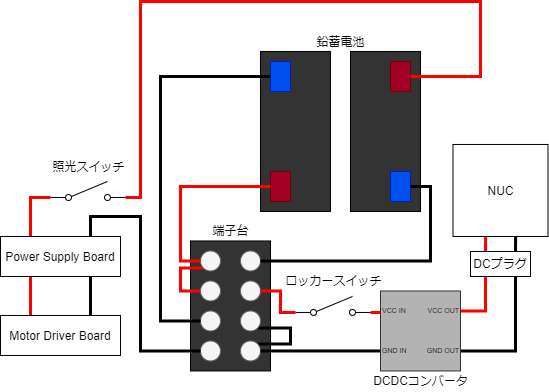
\includegraphics[width=100truemm, clip]{images/electrical_connections.png}
    \caption{Electrical Connection Diagram}
    \label{fig:electrical_connection_diagram}
  \end{figure}

  \subsection{端子の接続方法の詳細}

  \subsubsection{鉛蓄電池}
  鉛蓄電池WP20-12IEはM5ねじの接続端子を持っているので,Y型圧着端子をねじ止めすることで接続することができます.  
  ねじの締結には8mm幅のレンチを使用できます.感電やショートに十分注意して作業してください.

  \begin{figure}[ht]
    \centering
    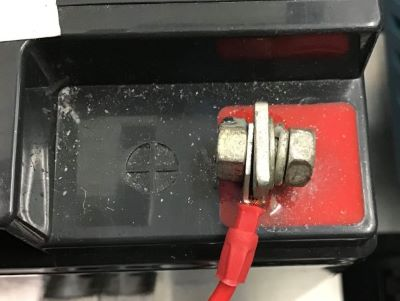
\includegraphics[width=65truemm, clip]{images/pb_battery.jpg}
    \caption{Detail of How to Connect Pb-Battery}
    \label{fig:pb_battery}
  \end{figure}

  \subsubsection{端子台}
  端子台ATK-30-6PはM5ねじの接続端子を持っているので,Y型圧着端子をねじ止めすることで接続できます.

  1つの端子に2つの圧着端子を接続することもできるので,圧着端子を両端につけたケーブルを使って2つの端子列をショートさせることができます.
  上の接続例でも,GNDや12Vの箇所でこのような接続方法をとっています.

  \begin{figure}[ht]
    \centering
    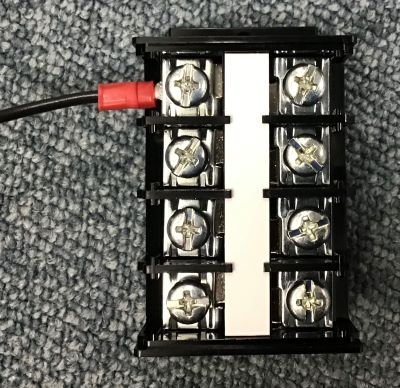
\includegraphics[width=65truemm, clip]{images/terminal.jpg}
    \caption{Detail of How to Connect Screw Terminal Block}
    \label{fig:terminal}
  \end{figure}

  \subsubsection{スイッチ}
  ADAMR2で使用しているスイッチは,いずれも187シリーズの差込型接続端子(ファストン端子)を持っています.
  接続には187シリーズの差込型端子(メス)を付けたケーブルを使用する必要があります.

  差込型接続端子ははんだ付け無しで何度も取り外しができますが,付け直す度に端子が摩擦で削れて接続が緩くなる可能性があります.
  取り外しはできるだけ最小限に抑えるよう注意してください.

  \begin{figure}[ht]
    \centering
    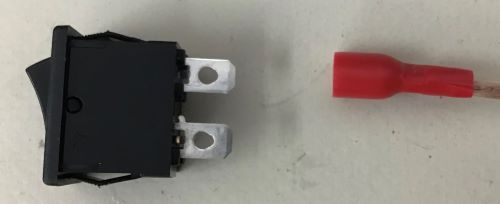
\includegraphics[width=65truemm, clip]{images/switch.jpg}
    \caption{Detail of How to Connect Switch}
    \label{fig:switch}
  \end{figure}

  \subsubsection{T-Frog電源基板}
  T-Frog電源基板は,M3ねじ止めターミナルを持っています.
  接続には内径φ3.2の圧着端子を使用します.ADAMR2では丸形圧着端子を使用しています.

  \begin{figure}[ht]
    \centering
    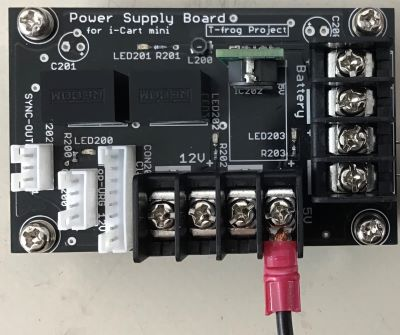
\includegraphics[width=65truemm, clip]{images/t-frog.jpg}
    \caption{Detail of How to Connect T-Frog Power Supply Board}
    \label{fig:t-frog}
  \end{figure}
\end{document}